\documentclass{sigchi}
\usepackage{xspace}
\usepackage{fancyvrb}
\usepackage{inconsolata}
\usepackage{xcolor}
\usepackage{tikz}
\newcommand*{\priority}[1]{\begin{tikzpicture}[scale=0.12]%
    \draw (0,0) circle (1);
    \fill[fill opacity=1,fill=black] (0,0) -- (90:1) arc (90:90-#1*3.6:1) -- cycle;
    \end{tikzpicture}}
\newcommand*{\priorityc}[1]{
\resizebox{0.8em}{0.8em}{
  {\protect\tikz{ \protect
    \draw[line width=1mm, black] (0,0) circle (1); \fill[fill opacity=1,fill=black] (0,0) -- (90:1) arc (90:90-#1*3.6:1) -- cycle;
    } }}}

\definecolor{kvdclr}{rgb}{0.3,0.0,0.8}
\DefineVerbatimEnvironment{thegamma}{Verbatim}{fontfamily=zi4,numbers=left,xleftmargin=6mm,fontsize=\small,commandchars=\\\{\}}
%\newcommand{\kvd}[1]{\textcolor{kvdclr}{#1}}
\newcommand{\kvd}[1]{\textbf{#1}}
\newcommand{\ikvd}[1]{{\fontfamily{zi4}\selectfont\small #1}}
\newcommand{\tg}{The Gamma\xspace}

% Use this section to set the ACM copyright statement (e.g. for
% preprints).  Consult the conference website for the camera-ready
% copyright statement.

% Copyright
\CopyrightYear{2020}
%\setcopyright{acmcopyright}
\setcopyright{acmlicensed}
%\setcopyright{rightsretained}
%\setcopyright{usgov}
%\setcopyright{usgovmixed}
%\setcopyright{cagov}
%\setcopyright{cagovmixed}
% DOI
\doi{https://doi.org/10.1145/3313831.XXXXXXX}
% ISBN
\isbn{978-1-4503-6708-0/20/04}
%Conference
\conferenceinfo{UIST'20,}{October  20--23, 2020, Minneapolis, MN, USA}
%Price
\acmPrice{\$15.00}

% Use this command to override the default ACM copyright statement
% (e.g. for preprints).  Consult the conference website for the
% camera-ready copyright statement.

%% HOW TO OVERRIDE THE DEFAULT COPYRIGHT STRIP --
%% Please note you need to make sure the copy for your specific
%% license is used here!
% \toappear{
% Permission to make digital or hard copies of all or part of this work
% for personal or classroom use is granted without fee provided that
% copies are not made or distributed for profit or commercial advantage
% and that copies bear this notice and the full citation on the first
% page. Copyrights for components of this work owned by others than ACM
% must be honored. Abstracting with credit is permitted. To copy
% otherwise, or republish, to post on servers or to redistribute to
% lists, requires prior specific permission and/or a fee. Request
% permissions from \href{mailto:Permissions@acm.org}{Permissions@acm.org}. \\
% \emph{UIST '20},  October 20--23, 2020, Minneapolis, MN, USA \\
% ACM xxx-x-xxxx-xxxx-x/xx/xx\ldots \$15.00 \\
% DOI: \url{http://dx.doi.org/xx.xxxx/xxxxxxx.xxxxxxx}
% }

% Arabic page numbers for submission.  Remove this line to eliminate
% page numbers for the camera ready copy
% \pagenumbering{arabic}

% Load basic packages
\usepackage{balance}       % to better equalize the last page
\usepackage{graphics}      % for EPS, load graphicx instead
\usepackage[T1]{fontenc}   % for umlauts and other diaeresis
\usepackage{txfonts}
\usepackage{mathptmx}
\usepackage[pdflang={en-US},pdftex]{hyperref}
\usepackage{color}
\usepackage{booktabs}
\usepackage{textcomp}

% Some optional stuff you might like/need.
\usepackage{microtype}        % Improved Tracking and Kerning
% \usepackage[all]{hypcap}    % Fixes bug in hyperref caption linking
\usepackage{ccicons}          % Cite your images correctly!
% \usepackage[utf8]{inputenc} % for a UTF8 editor only

% If you want to use todo notes, marginpars etc. during creation of
% your draft document, you have to enable the "chi_draft" option for
% the document class. To do this, change the very first line to:
% "\documentclass[chi_draft]{sigchi}". You can then place todo notes
% by using the "\todo{...}"  command. Make sure to disable the draft
% option again before submitting your final document.
\usepackage{todonotes}

% Paper metadata (use plain text, for PDF inclusion and later
% re-using, if desired).  Use \emtpyauthor when submitting for review
% so you remain anonymous.
\def\plaintitle{The Gamma: Data Exploration through Iterative Prompting}
\def\plainauthor{First Author, Second Author, Third Author,
  Fourth Author, Fifth Author, Sixth Author}
\def\emptyauthor{}
\def\plainkeywords{Data exploration; End-user programming; Data journalism; Programming languages; Type providers}
\def\plaingeneralterms{Documentation, Standardization}

% llt: Define a global style for URLs, rather that the default one
\makeatletter
\def\url@leostyle{%
  \@ifundefined{selectfont}{
    \def\UrlFont{\sf}
  }{
    \def\UrlFont{\small\bf\ttfamily}
  }}
\makeatother
\urlstyle{leo}

% To make various LaTeX processors do the right thing with page size.
\def\pprw{8.5in}
\def\pprh{11in}
\special{papersize=\pprw,\pprh}
\setlength{\paperwidth}{\pprw}
\setlength{\paperheight}{\pprh}
\setlength{\pdfpagewidth}{\pprw}
\setlength{\pdfpageheight}{\pprh}

% Make sure hyperref comes last of your loaded packages, to give it a
% fighting chance of not being over-written, since its job is to
% redefine many LaTeX commands.
\definecolor{linkColor}{RGB}{6,125,233}
\hypersetup{%
  pdftitle={\plaintitle},
% Use \plainauthor for final version.
%  pdfauthor={\plainauthor},
  pdfauthor={\emptyauthor},
  pdfkeywords={\plainkeywords},
  pdfdisplaydoctitle=true, % For Accessibility
  bookmarksnumbered,
  pdfstartview={FitH},
  colorlinks,
  citecolor=black,
  filecolor=black,
  linkcolor=black,
  urlcolor=linkColor,
  breaklinks=true,
  hypertexnames=false
}

% create a shortcut to typeset table headings
% \newcommand\tabhead[1]{\small\textbf{#1}}

% End of preamble. Here it comes the document.
\begin{document}

\title{\plaintitle}

\numberofauthors{1}
\author{%
  \alignauthor{Leave Authors Anonymous\\
    \affaddr{for Submission}\\
    \affaddr{City, Country}\\
    \email{e-mail address}}
}

\maketitle

\begin{abstract}
Governments, non-profit organizations and citizen initiatives publish increasing amounts of
data, but extracting insights from such data and presenting them to the public is hard.
First, data comes in a variety of formats that each requires a different tool. Second, many
data exploration tools do not reveal how a result was obtained, making it difficult to reproduce
the results and check how they were obtained.
%
We contribute The Gamma, a novel data exploration environment for non-experts. The Gamma is based
on a single interaction principle and using it results in transparent and reproducible scripts.
This allows transfer of knowledge from one data source to another and
learning from previously created data analyses. We evaluate the usability and learnability of
The Gamma through a user study on non-technical employees of a research institute.
%
We argue that the our approach allows journalists and the public to benefit from the rise
of open data, by making data exploration easier, more transparent and more reproducible.
\end{abstract}


% ACM Classfication
%
% \begin{CCSXML}
% <ccs2012>
% <concept>
% <concept_id>10003120.10003121</concept_id>
% <concept_desc>Human-centered computing~Human computer interaction (HCI)</concept_desc>
% <concept_significance>500</concept_significance>
% </concept>
% <concept>
% <concept_id>10003120.10003121.10003125.10011752</concept_id>
% <concept_desc>Human-centered computing~Haptic devices</concept_desc>
% <concept_significance>300</concept_significance>
% </concept>
% <concept>
% <concept_id>10003120.10003121.10003122.10003334</concept_id>
% <concept_desc>Human-centered computing~User studies</concept_desc>
% <concept_significance>100</concept_significance>
% </concept>
% </ccs2012>
% \end{CCSXML}
%
% \ccsdesc[500]{Human-centered computing~Human computer interaction (HCI)}
% \ccsdesc[300]{Human-centered computing~Haptic devices}
% \ccsdesc[100]{Human-centered computing~User studies}

% Author Keywords
\keywords{\plainkeywords}

% Print the classficiation codes
% \printccsdesc
% Please use the 2012 Classifiers and see this link to embed them in the text: \url{https://dl.acm.org/ccs/ccs_flat.cfm}

\begin{figure}
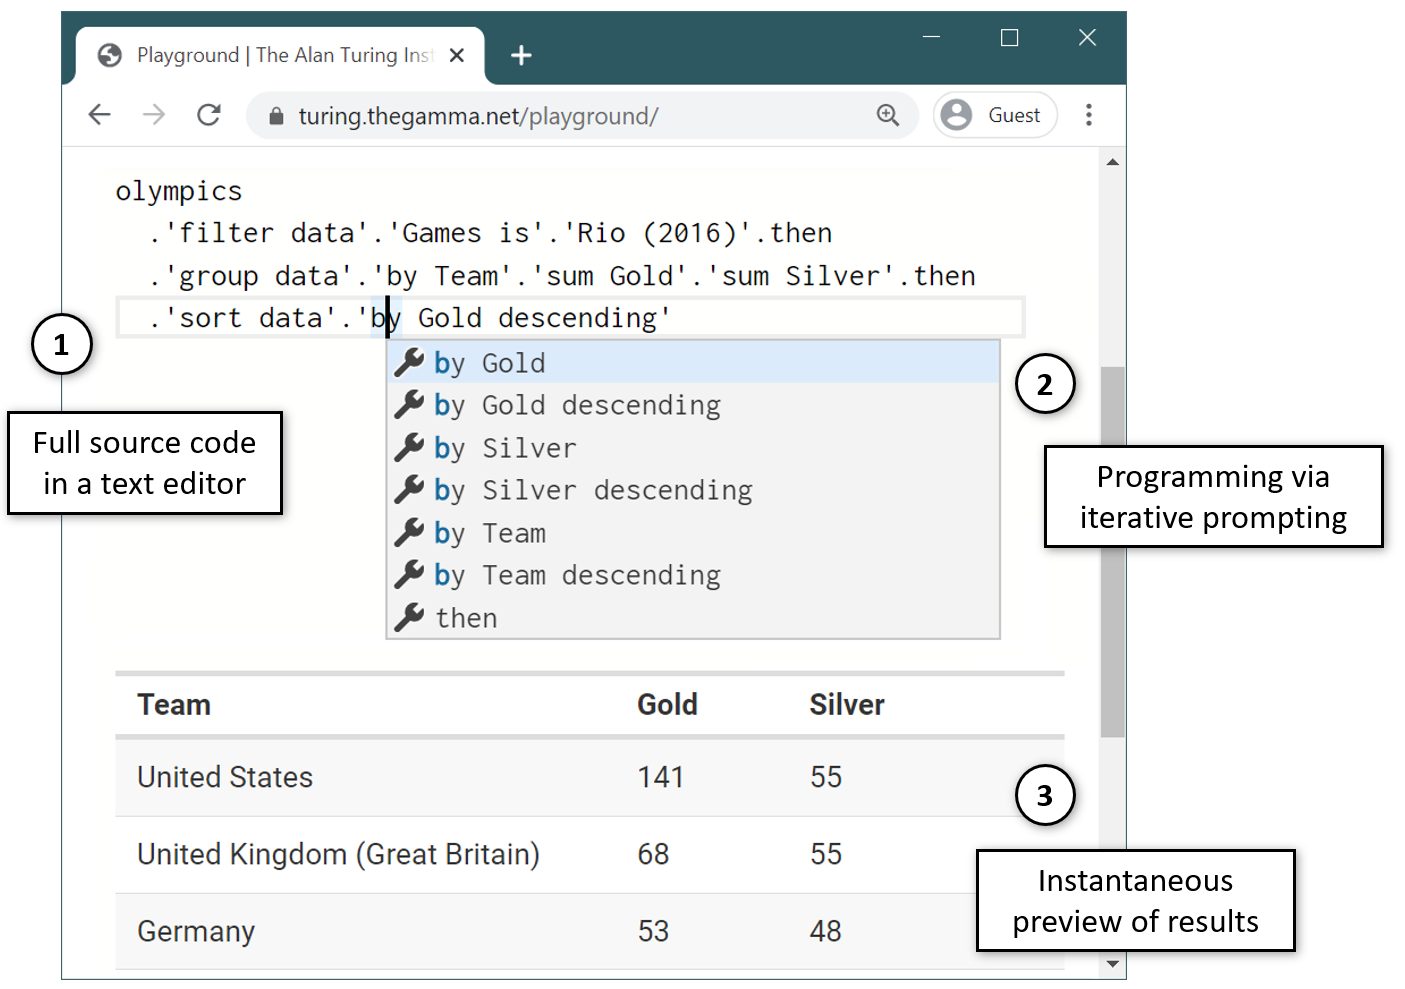
\includegraphics[width=1\columnwidth]{figures/thegamma-annot}
\caption{Teams with the greatest number of gold medals from Rio 2016
Olympics with a reproducible The Gamma script (1), an auto-complete prompt offering ways
of sorting the data (2) and instant preview (3).}
\label{fig:thegamma}
\vspace{-0.5em}
\end{figure}


\section{Introduction}
Data science has more capabilities to help us understand the world than ever before, yet at the
same time post-truth politics and increasing public distrust in statistics makes data-driven insights
increasingly less relevant in public discourse~\cite{howstatslost}. This should perhaps not be a surpirse.
Journalists can access increasing amounts of data, but producing engaging and transparent data-driven
reports that are easy to interpret is expensive and requires expert programming skills \cite{ddj}.

The design of a data exploration tool for journalists poses a unique mix of challenges. First, the
tool needs to be easy to learn for end-users working under tight deadlines. Second, it needs to
support a wide range of data sources in a way where the expertise gained when working with one data
source is relevant for other data sources. Third, the resulting data-driven insights need to be
transparent, allowing the readers to verify the claims and learn how to reproduce the work.

We present The Gamma, a text-based data exploration environment for non-experts. The Gamma
is based on a single interaction principle, which provides uniform
access to a range of data sources including data tables, graph databases and data cubes.
An anlysis created in The Gamma is a transparent script that can be followed to reproduce the
result from scratch. This allows learning from existing analyses and encourages readers
to engage with the results. Our key contributions are:

\begin{itemize}
\item We identify the design requirements for a data exploration tool for journalists
  (Section~\ref{sec:motivation}) and follow those to build a novel programming environment
  The Gamma (Section~\ref{sec:overview}).

\item We introduce \emph{iterative prompting} (Section~\ref{sec:design}),
  an interaction design principle that can be used to complete a variety of programming
  tasks in a uniform way that allows transfer of knowledge between different tasks.

\item We show how to use the iterative prompting principle for querying of distinct data
  sources including data tables, graph databases and data cubes (Section~\ref{sec:implementation}).

\item We discuss a number of case studies (Section~\ref{sec:cases}) and
  conduct a user study to evaluate the usability of The Gamma and the extent to which users can,
  (i) learn from examples and (ii)~transfer knowledge between tasks (Section~\ref{sec:study}).
\end{itemize}

The Gamma is available as open-source at \href{http://thegamma.net}{\small\bf\ttfamily thegamma.net}.

\section{Related work}

The Gamma brings together recent programming language innovations for working with data
\cite{inforich}, work on making programming accessible to non-programmers \cite{enduser,smallmatter}
and work on tools for journalists such as Idyll \cite{idyll}. Related work includes a range of
visual and programmatic tools used by data scientists, work that aims to simplify programming
or explore alternative paradigms and various predictive tools that assist users in completing
programming or data exploration tasks.

% Evaluating ui systems research
% \cite{evaluating}

\subsection{Data science tools}
Data exploration is typically done using spreadsheets, comprehensive visual tools or
via code using notebooks. Notebooks such as Jupyter \cite{jupyter} are also popular with technically
skilled journalists as they allow combining code with commentary and visual outputs. However,
notebooks can lead to messy hard to reproduce code \cite{messes,wrattler}.

Visual data analytics tools \cite{control,vizdom} such as Tableau \cite{tableau} do not require
programming skills, but require mastering a range of different interactions. They also make it
hard to see what data transformations have been done. Several systems for data exploration,
e.g.~Potter's Wheel and Wrangler \cite{potter,wrangler}, and visualization, e.g.~Lyra \cite{lyra},
provide a GUI, but record a transparent script that can be seen and modified by the user.

\subsection{Easier programming tools}
We aim to design a programming environment that is easy to use and learn. Many approaches to this
goal have been tried. Victor \cite{learnable,principle} introduced design principles that
inspired many to build live programming systems \cite{review,liveroad,lighttable} that give
immediate feedaback to help programmers understand how code relates to output and
exploratory systems \cite{variolite,exploratory} that assist with completing open-ended tasks.

To avoid difficulties with editing code as text, some systems use structured editors~\cite{structure-based,livenut,lamdu}.
In Subtext \cite{subtext,directprog} the language itself is co-designed with the editor to make
the interactions with code more natural. Finally, programming can be made easier by designing
high-level declarative abstractions. Tea does so for statistical analyses \cite{tea} and
Satyanarayan et al. \cite{interactionviz,vegalite} does so for interactive data visualizations.

The Gamma is live in that it gives an instant preview of the results. It is text-based,
although it is syntactically simple. The code written in The Gamma is high-level and so work
on declarative abstractions is a valuable inspiration.

\subsection{Code completion and assistants}
A key component in The Gamma design is the use of auto-complete for offering possible
operations. Code completion has been pioneerd by Kaiser~\cite{assistants}, but our work is more
directly inspired by the work on type providers \cite{inforich,fsdata,dotdriven}, which utilize
code completion to integrate external data into a statically typed programming language.

When using type providers, completions are offered as the user types code. However, completion
tools can also recmmend scripts when users begin interacting with data \cite{predictive,proactive}.
Alternatively, they can also be guided by natural language as for example Eviza~\cite{eviza},
which uses natural language for data exploration. CodeMend~\cite{codemend} uses natural language
for more general code edits, but uses data visualization as a case study.
Finally, data entry interfaces based on completion such as Dasher \cite{dasher} utilize an
interaction principle similar to our iterative prompting.

\subsection{Programming without writing code}

A number of tools for data exploration use alternative approaches to programming where
the user does not write code. In programming by example \cite{byexample}, the user gives
examples of desired results. In data science, this approach has been used for example for
specifying data transformations in spreadsheets and data extraction \cite{spreadsheetpbe,flashextract}.

In direct manipulation \cite{direct}, a program is specified by directly interacting with the
output. This has been used in the visual domain \cite{sketchnsketch}, but also for data querying
\cite{dynamicq,vlang}. The VQE language~\cite{visage} also considers how to allow code reuse and
modification in this context. Direct manipulation can also support data exploration by letting
users partially edit queries,~e.g. by changing quantifiers as in DataPlay~\cite{dataplay}.

\newpage


\begin{figure}
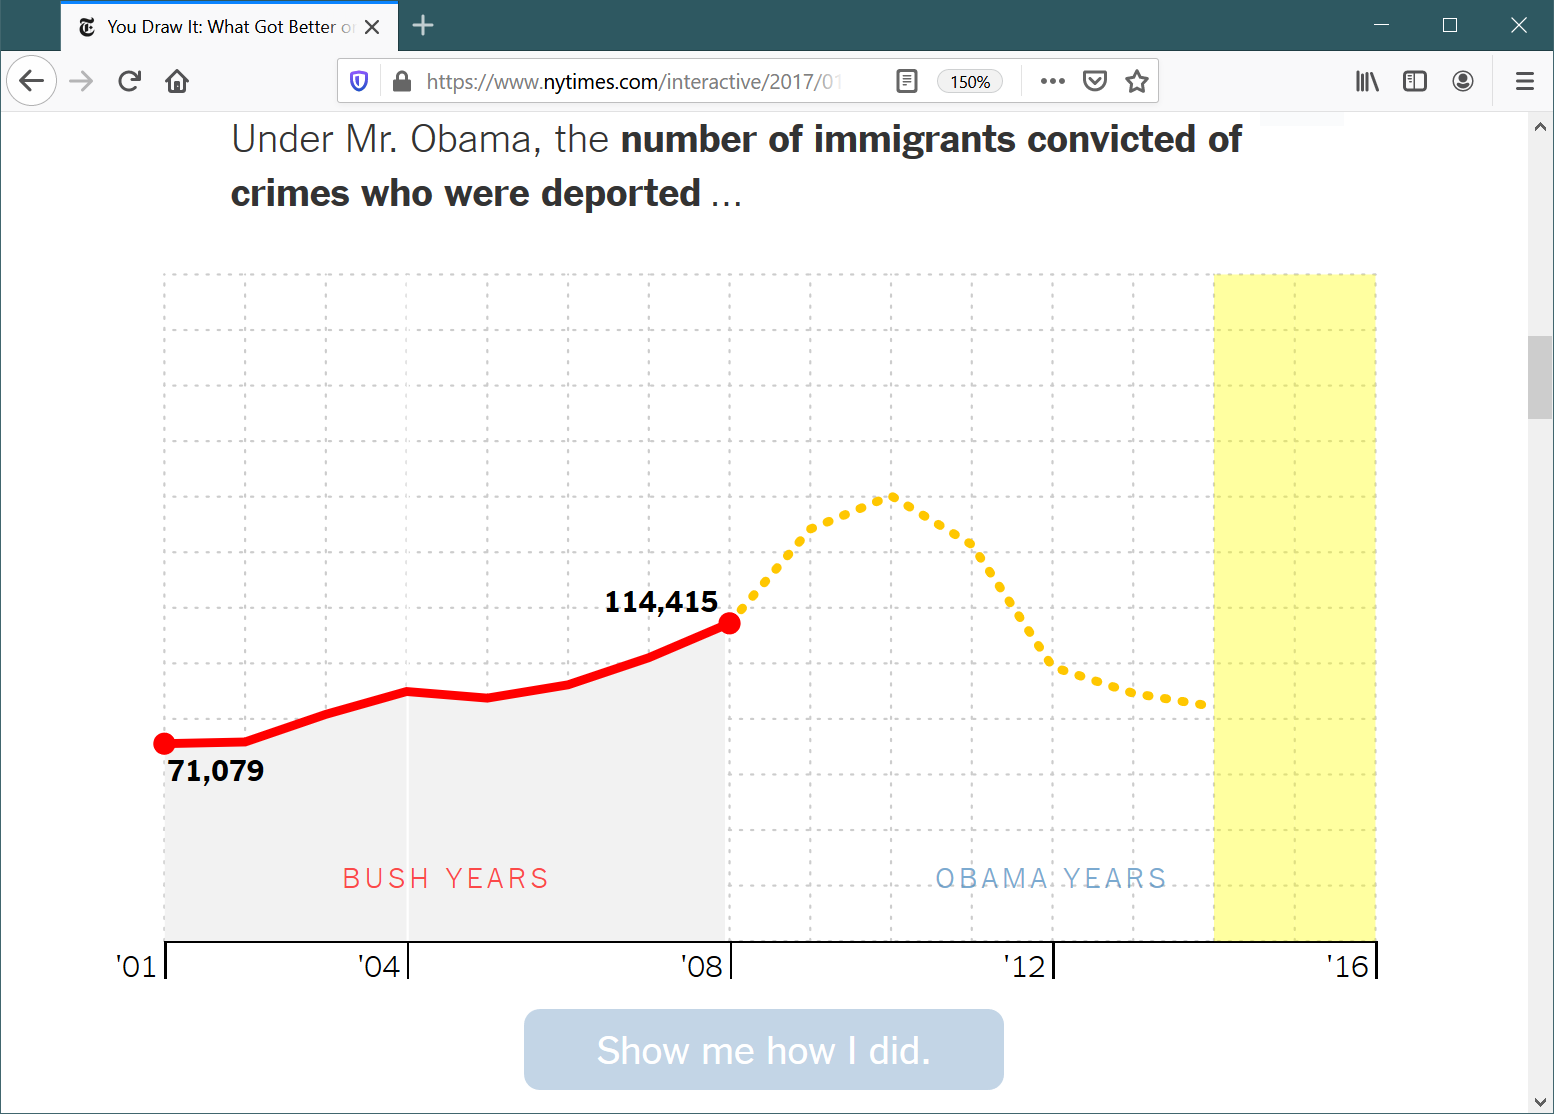
\includegraphics[width=1\columnwidth]{figures/nyt}
\caption{New York Times article on Obama's legacy \cite{youdraw}. The article asks the reader to make a guess
(engagement), but only lists ``Immigration and Customs Enforcement'' as a source of data.}
\label{fig:nyt}
\end{figure}

\section{Motivation}
\label{sec:motivation}

The Gamma aims to adapt the recent innovations in programming language research, especially the
work on type providers, into a form where it could be used in practice by journalists and other
non-expert interested in data exploration. We start with a careful consideration of our target
application domain, i.e.~data analyses produced by journalists and citizen data scientists that
are published online. We look at both practical requirements for such programming environment
and requirements arising from our focus on journalism. This analysis is based on the author's
experience of collaborating with journalists\footnote{Citations removed to preserve anonymity.},
review of literature on data journalism, e.g.~\cite{ddj,edcj17,edcj18} and more general trends in
journalism.

\subsection{Open Journalism}
Journalism continually develops and responds to the many challenges it faces \cite{future}.
Two recent challenges are relevant to our work. The first is building trust in media.
One way of establishing trust in the age of fake news is to be more transparent about editorial
decisions, process and original sources. Many journalists believe that opening up the process
shows the quality and trustworthiness of their work~\cite{transparency}.
The second challenge is reader engagement. To develop a relationship with readers, journalists are
increasingly looking for meaningful ways of engagement. This includes reader comments, involvement
of citizen journalists \cite{comments,citizen} and the development of new interactive formats
\cite{youdraw}. To address the above challenges, a tool for data exploration should satisfy the
following three requirements.

\paragraph{Trust Through Transparency}
To support trustworthiness, data analyses should be transparent. The reader should be able to
determine what is the source of analysed data and how has the data been transformed. As much as
possible, these capabilities should also be accessible to non-expert readers.

\paragraph{Reproducibility for Fact Checking}
It should be possible to re-run the analysis to verify that it produces the presented results.
However, running an opaque script is not enough. A reader should be able to recreate the analysis
by following the necessary steps from the original data source to the end result.

\paragraph{Encouraging Meaningful Engagement}
The tool should support a mechanism through which readers can engage in a meaningful discussion.
For example, it should allow modifying of parameters of a data visualization in order to show
how different choices affect the final result.

\begin{figure}
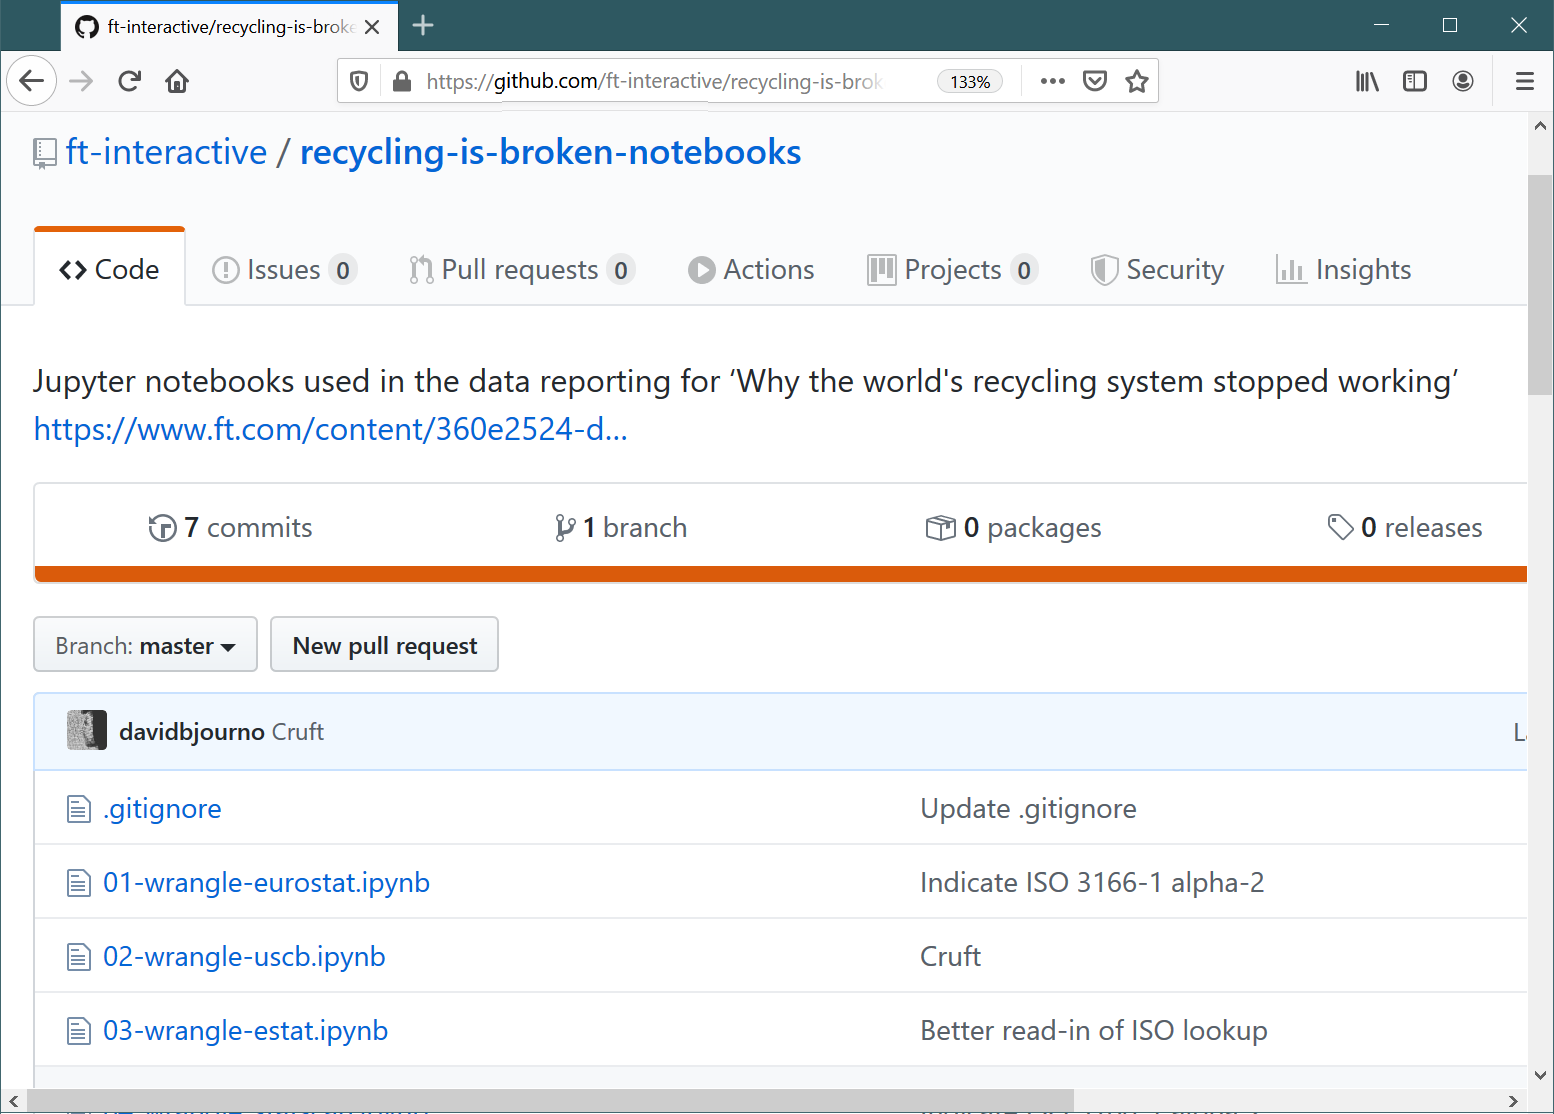
\includegraphics[width=1\columnwidth]{figures/ft}
\caption{Financial Times analysis of recyclable waste. Full source is provided as Jupyter Notebooks
on GitHub \cite{ftnotebooks}, but re-running the analysis is difficult, even for an expert.}
\label{fig:ft}
\end{figure}

\subsection{End-user Data Exploration}
Our aim is to make programmatic data exploration accessible to journalists, but we want to keep
the desirable properties of text-based programming. In particular, source code of a data
exploration should provide a full reproducible record of how the data analysis has been done.
As end-users, journalists have a number of interesting characteristics. They work under tight
deadline and data exploration is only a complementary skill. They also need to work with a wide
range of data sources, including big data tables (e.g.~Iraq War documents leak) or graph
databases (e.g.~Panama Papers). This leads to a number of practical requirements on the programming
environment.

\paragraph{Conceptual Simplicity}
We target end-users who cannot dedicate much time to learning about a tool prior
to using it. Consequently, using the tool should require understanding of only a small number
of concepts. Once the user understand a small number of concepts, they should be able to complete
basic data exploration tasks.

\paragraph{Uniformity across Data Sources}
The users should be able to navigate through large databases, query relational databases and
query graph databases through the same mechanism. Ideally, expertise gained with one data source
should also be transferable to working with another data source.

\paragraph{Learning without Experts}
Sarkar \cite{learning} reports that users learn how to use Excel either by talking to experts,
or by seeing a feature in a spreadsheet received from a colleague. In our circumstances, experts
are unlikely to be available, so the tool should support learning from examples. When looking at
a work done and published by another person, the user needs to see (and be able to understand)
how a task was completed.

\newpage
~
\newpage


\section{Overview}
\label{sec:overview}

\tg is a text-based programming environment that allows non-experts create simple data exploration
scripts using a single interaction principle -- choosing an item from an auto-complete list.
It supports a range of data sources including tabular data, graph data and data cubes.

\subsection{Querying Travel Expenses}
To introduce \tg, we walk through a simple problem that a local journalist might want to solve.
The UK government publishes travel expense claims by members of the House of Lords. A journalist
wants to find out which of the members representing the Kent county spend the most on travel.
The following shows a subset of the data:\footnote{ \url{https://www.parliament.uk/mps-lords-and-offices/members-allowances/house-of-lords/holallowances/} }

\begin{thegamma}
\textbf{Name, County, Days Attended, Days Away, Travel Costs}
Lord Adonis, London, 8, 0, 504
Baroness Afshar, Yorkshire, 2, 0, 0
Lord Alderdice, Oxfordshire, 3, 0, 114
Lord Alli, London, 5, 0, 0
Baroness Amos, London, 3, 0, 0
\end{thegamma}

After the analyst imports the CSV file (through a web interface), the environment is initialized
with code that refers to the imported variable \ikvd{expenses}. The analyst then types `.' (dot):

\begin{thegamma}
expenses.
\end{thegamma}
\vspace{-0.4em}\qquad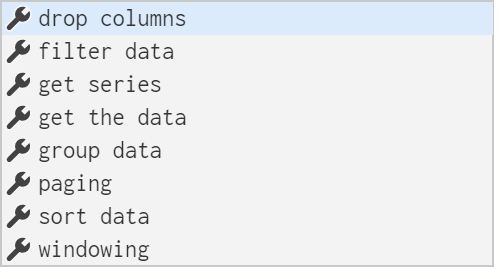
\includegraphics[width=0.5\columnwidth]{figures/lords1}

The type provider for tabular data allows analysts to construct simple queries. It first offers
a list of operations that the analyst might want to perform such as grouping, filtering and sorting.
To find members of the House of Lords from Kent, the analyst chooses \ikvd{filter data},
types `.' and then chooses \ikvd{County is} from the offered list, types `.' and starts
typing Kent:

\begin{thegamma}
expenses
  .'filter data'.'County is'.Ke
\end{thegamma}
\vspace{-0.4em}\qquad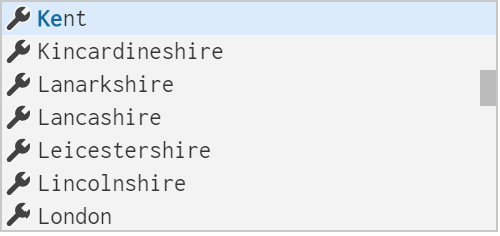
\includegraphics[width=0.5\columnwidth]{figures/lords2}

The completion list is generated from the values in the \ikvd{County} column of the dataset.
After selecting \ikvd{Kent}, the live preview is updated to only show records according to the
specified filter:

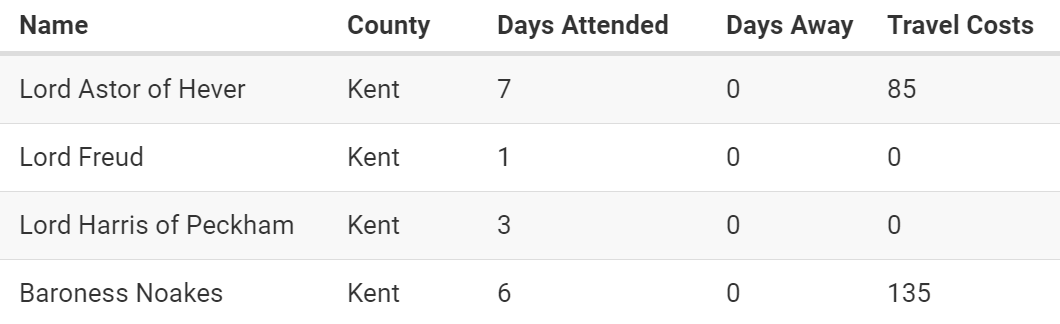
\includegraphics[width=1\columnwidth]{figures/lords3}

To finish specifying filtering conditions, the analyst chooses \ikvd{then} and is offered the
same list of querying operations as in the first step. To sort House of Lords members by their
travel costs, she now chooses \ikvd{sort data} and types `.' (dot):

\begin{thegamma}
expenses
  .'filter data'.'County is'.Kent.then
  .'sort data'.
\end{thegamma}
\qquad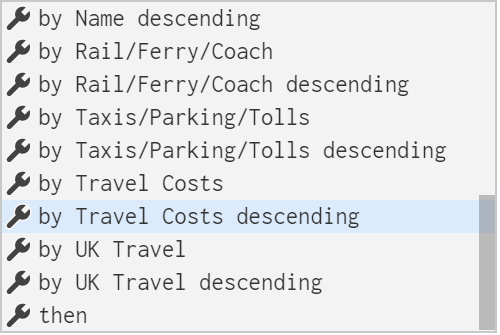
\includegraphics[width=0.5\columnwidth]{figures/lords4}

The auto-complete offers a list of columns that can be used for sorting, each with ascending
(default) and descending order option. After choosing one or more sort keys, the analyst selects
the \ikvd{then} member and is, again, offered the list of querying operations. They use
\ikvd{paging} to get top 5 records and \ikvd{get series} to obtain a data series with just
the House of Lords member name and their travel expenses.

\begin{thegamma}
expenses
  .'filter data'.'County is'.Kent.then
  .'sort data'.'by Travel Costs descending'.then
  .paging.take(5)
  .'get series'.'with key Name'.'and value Travel Costs'
\end{thegamma}

When the code evaluates to a data series with a categorical (textual) key and a numerical value,
\tg switches from displaying the result as a table to a column chart:

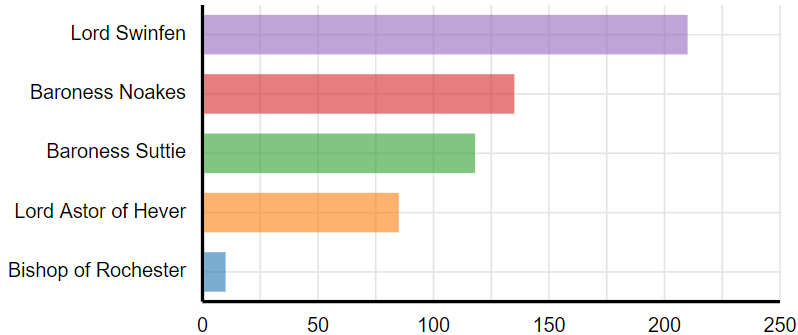
\includegraphics[width=1\columnwidth]{figures/lords5}
\vspace{-1.5em}

\subsection{Querying via Iterative Prompting}
In the example, the journalists constructs a query that filters and sorts a data table. This is
not unlike writing a query in the SQL language. However, the whole query is constructed through
a single interaction mechanism that we refer to as \emph{iterative prompting}. The user triggers
the interaction by typing `.' at the end of the query constructed so far. She is then offered a
list of available operations in the current context. This may include a choice of top-level
operations (e.g.~at the start and then again after choosing \ikvd{then}) or possible
parameters for an operation (such as possible sorting keys and directions after choosing
\ikvd{sort data}). The user then merely needs to choose one of the available options, rather than
learning the syntax and semantics of SQL in order to know what constructs can be used in the
given context.
We discuss the important aspects of The Gamma design in the next section and then discuss the
integration of specific data sources in detail, revisiting the type provider for querying
data tables.

% ==================================================================================================

\section{Design}
\label{sec:design}

We identified a number of requirements for a data exploration tool for journalists earlier.
First, using the tool should result in transparent and reproducible data analyses that can be
understood and modified by non-experts. Second, the tool should minimze the number of concepts
that the user needs to understand and, subsequently, allow them to learn through exploration
and from examples. In this section, we discuss how our design aims to satisfy those requirements.

\subsection{Lowering the Barrier to Entry}
Data exploration tasks, such as querying tables, have a certain irreducible complexity.
Regardless of the interface, the user will be exposed to concepts such as filtering,
sorting and grouping. Our design aims to lower the barrier to entry by stratifying the concepts
into first-level \emph{iterative prompting} principle and second-level \emph{domain specific
languages} for each kind of data source.
The user needs to master the iterative prompting principle in order to start working
with the system. However, using individual data sources can be mastered gradually.

\paragraph{Iterative Prompting}
Iterative prompting is an interaction principle where the user repeatedly invokes an
auto-complete prompt and makes a selection from the offered options. The principle is closely
related to both code completion and the use of command line. Iterative prompting is novel as an
overarching interaction principle for program construction.

In code completion, the auto-complete
prompt is invoked only in certain contexts, e.g.~when accessing a member of an object through a
variable defined earlier in code. It requires the user to be sufficiently familiar with the
programming language in order to get to a point where they are offered a list of members. In
contrast, our system only requires choosing the initial data source. The rest of the programming
is done via iterative prompting. The iterative nature of iterative prompting makes it similar to
using the command line or REPL (read-eval-print-loop) tools. However, those repeatedly ask the
user to type code or commands.

%https://www.nngroup.com/articles/recognition-and-recall/
We argue that iterative prompting is easier than other forms of interaction, because it
follows the \emph{recognition over recall} usability heuristic. The users are only required to
choose from an offered list of options, rather than having to recall a possible command
(to type in a command line) or a syntax in a text-based programming environment.

\paragraph{Domain Specific Languages}
The access to individual data sources in The Gamma is facilitated through a domain specific
language, which defines the primitives that are offered to the user in the auto-complete prompts
invoked through iterative prompting. The domain specific languages are embedded in The Gamma --
they define merely the available members (and specify how to evaluate a chain of members), but
they cannot define any custom syntax.

We discuss the individual domain specific languages for querying data tables, graph databases and
data cubes in a later section. The complexity of those languages differs. The previously discussed
language for querying tabular data is the most complex one. However, The Gamma makes it easy for
the user to start exploring and learning new languages, because they are all accessible via
iterative prompting.

\subsection{Building the Magic Escalator of Knowledge}
As discussed earlier, The Gamma is designed for users who work under tight deadlines and only
analyse data as their secondary task. The Gamma aims to support such users by having a low
barrier for entry and making it easy to learn independently.

\paragraph{Design for Percolation}
When analysing how Excel users learn Sarkar \cite{learning} points out that users learn new
features opportunistically when the usage of a feature is apparent in a spreadsheet. For
example, users can learn different functions to use in formulas, because those are visible in
the cell. Learning how to use a wizard for creating charts in this way is not possible because
it leaves no trace in the spreadsheet -- only the final result. Sarkar's recommendation is to
\emph{design for percolation}, i.e.~in a way where looking at the final result makes it apparent
what feature has been used and how.

\paragraph{Text-based Source Code}
In The Gamma, each step in the iterative prompting process results in an identifier that is
added to the source code. This means that a program constructed solely through iterative prompting
keeps a full trace of how it was created. Seeing the resulting source code provides the user all
information that they need to recreate the program, not just by copying it, but also by using the
iterative prompting mechanism. The Gamma represents code as text and allows the user to edit it
freely, so not all interactions leave a trace. For example, deleting the most recently selected
option and choosing a different one is not apparent from the result.

\subsection{Making Complex Things Possible}
Although the focus on The Gamma is simple data exploration and almost all the use cases we
envision can be achieved using the iterative prompting interaction principle, there remain a
few cases where more flexibility is needed. We aim to \emph{make simple things easy and
complex things possible}. The language thus supports a small number of additional constructs that
can only be used through text editing. The following example illustrates three additional
constructs:

\begin{thegamma}
\kvd{let} topTravel =
  expenses
    .'sort data'.'by Travel Costs descending'.then
    .paging.take(5).'get series'
    .'with key Name'.'and value Travel Costs'

charts.column(topTravel)
  .setTitle("House of Lords members by travel expenses")
  .setColors(["red","blue","green"])
\end{thegamma}

First, The Gamma allows operations with parameters such as \ikvd{take(3)} or \ikvd{setTitle("...")}.
This is currently needed when writing a query that skips or takes first N elements from a table.
The remaining features are not needed for basic data exploration, but allow other scenarios, such
as manual creation of charts. The \ikvd{let} construct can be used to define (immutable) variables
and The Gamma also supports lists written as \ikvd{[1,2,3]}.

% ==================================================================================================

\begin{figure}
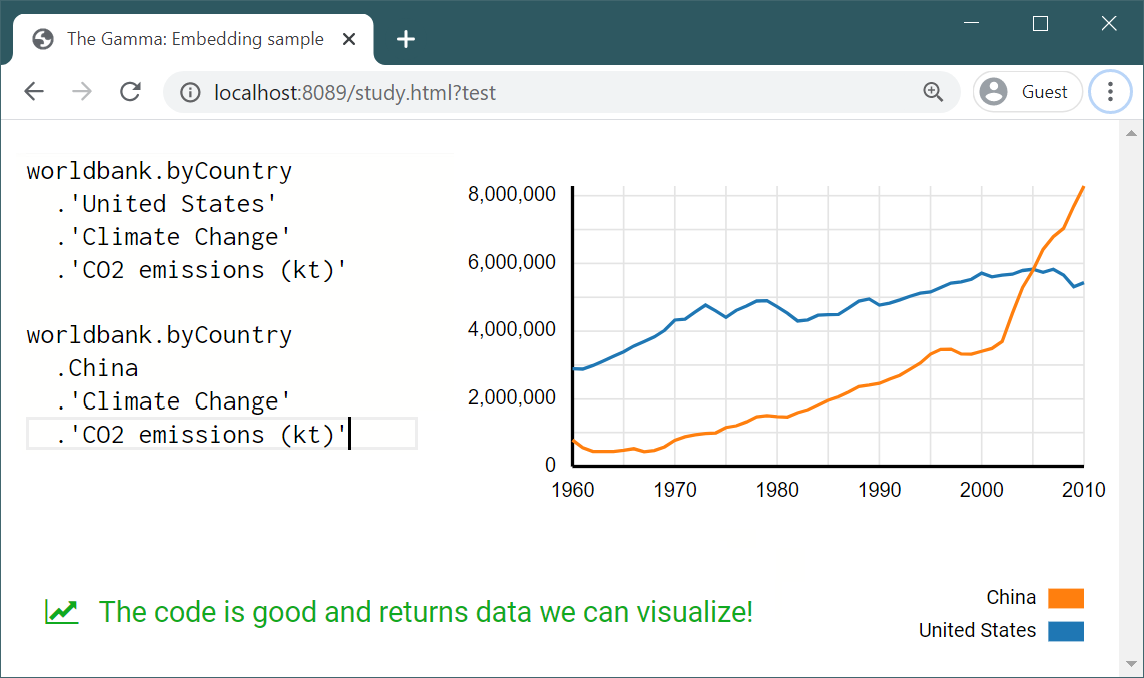
\includegraphics[width=1\columnwidth]{figures/sidebyside}
\caption{The Gamma environment with an automatically generated chart comparing CO2 emissions
of China and United States.}
\label{fig:sidebyside}
\end{figure}


\section{Implementation}
\label{sec:implementation}
The Gamma consists of a programming language with a web-based coding environment and a number
of type providers that provide access to various kinds of data sources. The system is implemented
in F\# and compiled to JavaScript using Fable.

\subsection{The Gamma Language}
In The Gamma, a program is a sequence of commands. A command can be either a variable declaration
or an expression that evaluates to a value such as a data table or a chart.
An expression is a reference to a data source followed by a chain of member accesses.
A member can be either an ordinary member or an operation which takes a list of parameters
enclosed in parentheses. When the member name contains non-alphanumerical characters such as
whitespcae, it needs to be written in quotes. Our implementation supports a few other features,
but those are not used in this paper.

The Gamma uses a type system to infer what members are available at a given point in a chain.
A type is an object with a list of members that, in turn, have their own types.
The types are not built-in, but are generated by a type providers for individual data sources.
The types are generated lazily and are only computed when a member appears in code.

The web-based coding environment uses the Monaco\footnote{\url{https://microsoft.github.io/monaco-editor/}}
editor and implemts auto-completion feature that is triggered when the user types `.' and relies
on information from the type system. The can display the value of a current command inline
as in Figure~\ref{fig:thegamma}, or values of all commands on the side as in Figure~\ref{fig:sidebyside}.
In the latter case, it can also combine one or more data series into a single chart.

\begin{figure}
\centering
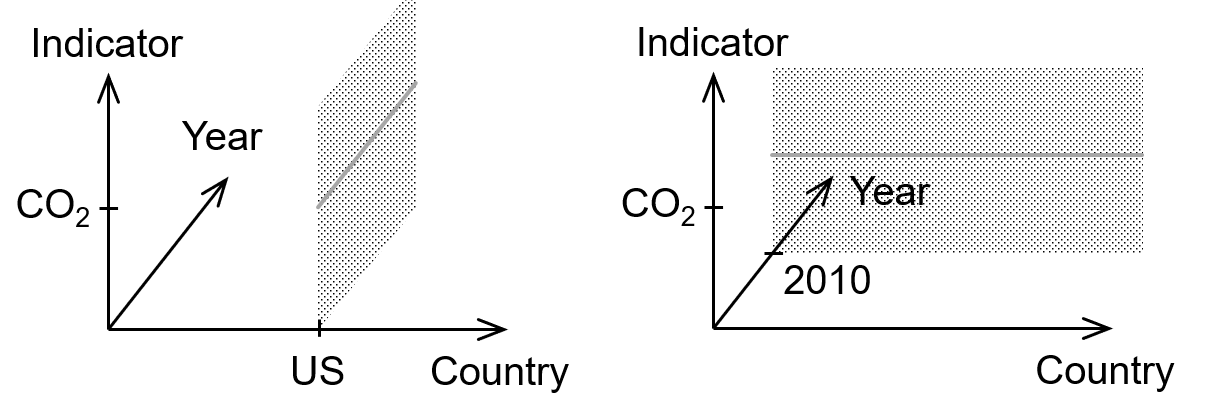
\includegraphics[scale=0.28]{figures/cubetp}
\caption{Exploring data cubes. The World Bank provider allows users to first choose
  a country or a year and then an indicator.}
\label{fig:cubetp}
\end{figure}

\subsection{Data Cube Type Provider}
Our first type provider allows users explore data form a data cube. For example, the World
Bank\footnote{\url{https://data.worldbank.org/}} collects a range of indicators about many
countries in the world each year. The data set is a three-dimensional cube with dimensions
corresponding to countries, indicators and years. The following example, also shown in
Figure~\ref{fig:sidebyside}, uses the provider to access CO2 emission data for United States:

\begin{thegamma}
worldbank.byCountry.'United States'
  .'Climate Change'.'CO2 emissions (kt)'
\end{thegamma}

As illustrated in Figure~\ref{fig:cubetp}, the provider allows uses to select a data series
from the data cube. By choosing \ikvd{byCountry.\textquotesingle United States\textquotesingle},
we restrict the cube to a two-dimensional plane. We then choose an indicator category
\ikvd{\textquotesingle Climate Change\textquotesingle} and a specific indicator
\ikvd{\textquotesingle CO2 emissions (kt)\textquotesingle}, obtaining a time series with
years as keys and emission data as values. The World Bank provider also supports filtering
by year and indicator.

Another type provider available in The Gamma that is based on the data cube structure allows
the user to explore UK government expenditure:

\begin{thegamma}
expenditure.byService.Defence.inTermsOf.GDP
\end{thegamma}

The dimensions of the cube are government services, years and value type (adjusted, nominal,
per GDP). Here, we select the \ikvd{Defence} service and \ikvd{GDP} value type. Our implementation
does not yet use a standardized data cube storage and so adding another data cube source
currently requires implementing a new type provider.

\subsection{Tabular Data Type Provider}

Our second type provider allows users to construct queries to explore data in tabular formats
such as CSV files. It is based on the theory developed Petricek~\cite{dotdriven}. Unlike the
data cube provider, the provider for tabular data does not just allow selecting a subset of the
data, but it can be used to construct SQL-like query. Consider the example from Figure~\ref{fig:thegamma}:

\begin{thegamma}
olympics.'filter data'.'Games is'.'Rio (2016)'.then
  .'group data'.'by Team'.'sum Gold'.'sum Silver'.then
  .'sort data'.'by Gold descending'
\end{thegamma}

The example works with a CSV file that records individual medals awarded in Olympic games.
The chain constructs a query that selects rows corresponding to the Rio 2016 Olympics and then
calculates total number of gold and silver medals for each team (country) before sorting the data.

When using the provider, the user specifies a sequence of operations. Members such as
\ikvd{\textquotesingle filter data\textquotesingle} or \ikvd{\textquotesingle group data\textquotesingle}
determine the operation type. Those are followed by operation parameters. For example, when grouping
data, we first select the key and then add a number of aggregations to calculate over the group.
Unlike SQL, the provider only allows users to choose from pre-defined aggregations such as
calculating the sum, average or the number of distinct values. As illustrated in
Section~\ref{sec:cases}, this still allows us to construct a wide range of practical queries.


\begin{figure}
\centering
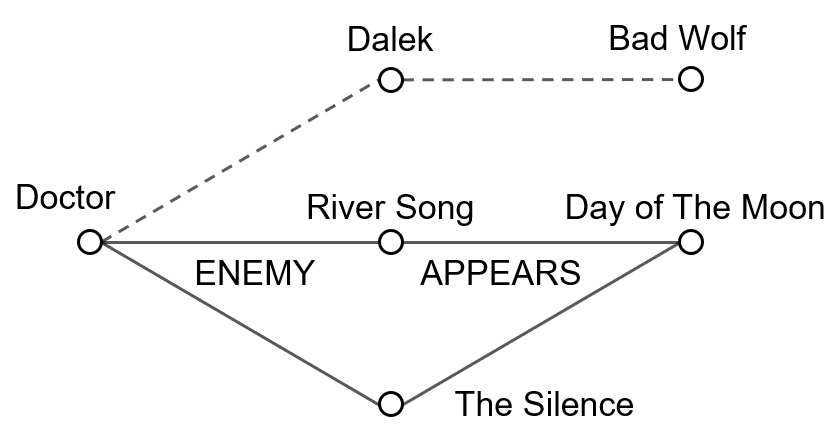
\includegraphics[scale=0.28]{figures/graphtp}
\vspace{0.5em}
\caption{Exploring graph databases. The user specifies a path through the data, possibly with
  placeholders to select multiple nodes.}
\label{fig:graphtp}
\end{figure}

\subsection{Graph Database Type Provider}
Our third type provider allows users explore data from graph databases. A graph database
consists of nodes representing entities and relationships between them. In the context of
data journalism, graph databases have been used for example in The Panama Papers reporting \cite{panama}.

The following example explores a database of Doctor Who characters and episodes. It retrieves
all enemies of the Doctor that appear in the Day of the Moon episode:

\begin{thegamma}
drwho.Character.Doctor
  .'ENEMY OF'.'[any]'
  .'APPEARED IN'.'Day of the Moon'
\end{thegamma}

We start from the \ikvd{Doctor} node and then follow two relationships. We use
\ikvd{\textquotesingle ENEMY OF\textquotesingle.\textquotesingle [any]\textquotesingle}
to follow links to all enemies of the Doctor and then specify
\ikvd{\textquotesingle APPEARED IN\textquotesingle.\textquotesingle Day of the Moon\textquotesingle}
to only select only such enemies that appear in a specific episode. The resulting query
is illustrated in Figure~\ref{fig:graphtp}.

The provider works with any graph database and generates members automatically, based on the
data in the database. In the above example, \ikvd{ENEMY OF} and \ikvd{APPEARED IN} are labels
of relations and \ikvd{Doctor} and \ikvd{Day of the Moon} are labels of nodes. The
\ikvd{[any]} member defines a placeholder that can be filled with any node with the specified
relationships. The results returned by the provider is a table of properties of all nodes
along the specified path. As discussed in the next section, such table can be further queried
using the tabular data type provider.

% ==================================================================================================


\section{Use cases}
\label{sec:cases}

The Gamma aims to simplify programmatic data exploration while keeping enough expressive power
to allow users to create interesting data visualizations. We consider the expressive power in
this section and assess simplicity in the next one. We used The Gamma to analyse
the UK government expenditure, activities of a research institute, Olympic medals and
information about the Doctor Who series\footnote{Links removed to preserve anonymity.}.
In this section, we consider two interesting larger examples.

\subsection{If Michael Phelps were a Country}
Michael Phelps has won so many medals that media compared him to
countries.\footnote{\href{https://www.npr.org/sections/thetorch/2016/08/14/489832779/}{\small\bf\ttfamily npr.org/sections/thetorch/2016/08/14/489832779/}}
Using the tabular data provider, we construct a chart shown in Figure~\ref{fig:cases} that
produces a country league table including Michael Phelps:\footnote{Available at: \url{http://gallery.thegamma.net/86/}}

\begin{thegamma}
\kvd{let} data = olympics
    .'group data'.'by Team'.'sum Gold'.then
    .'sort data'.'by Gold descending'.then
    .paging.skip(43).take(4)
    .'get series'.'with key Team'.'and value Gold'

\kvd{let} phelps = olympics
  .'filter data'.'Athlete is'.'Michael Phelps'.then
  .'group data'.'by Athlete'.'sum Gold'.then
  .'get series'.'with key Athlete'.'and value Gold'

charts.bar(data.append(phelps))
  .setColors(["#aec7e8","#aec7e8","#1f77b4"])
\end{thegamma}

The core of the data analysis is done in two commands. The first counts gold medals by countries
and uses paging to fetch 4 countries with suitable number of medals. In the second, we abuse the
grouping operation to aggregate data for just a single group. The two data series are then assigned
to local variables (for readability) and passed to the \ikvd{chart.columns} function.
In this case study, the core data exploration can be constructed via iterative prompting, but
building a chart requires invoking the \ikvd{append} operation and specifying colors using a list.

\subsection{The Most Frequent Doctor Who Villains}
In the second case study, we list Doctor Who villains by the number of episodes in which they
appear.\footnote{Available at: \url{http://gallery.thegamma.net/87/}} This is interesting as it
combines the graph database provider for fetching the data with the tabular data provider for
summarization:

\begin{thegamma}
\kvd{let} topEnemies = drWho.Character.Doctor
  .'ENEMY OF'.'[any]'.'APPEARED IN'.'[any]'.explore
  .'group data'.'by Character name'
    .'count distinct Episode name'.then
  .'sort data'.'by Episode name descending'.then
  .paging.take(8).'get series'
    .'with key Character name'.'and value Episode name'

chart.bar(topEnemies)
\end{thegamma}

Lines 1-2 use the graph database provider to find all paths linking the Doctor node with any
character linked via \ikvd{ENEMY OF}, followed by any episode linked by \ikvd{APPEARED IN}.
This produces a table that can be analysed using the tabular data provider by choosing the
\ikvd{explore} member. For each character (the villain) we count the total number of
distinct episodes in the table. The result is shown in Figure~\ref{fig:cases}.

The logic is not trivial, but it performs a fairly sophisticated data analysis that involves a
graph database query followed by an SQL-like data aggregation. The code can be constructed
using iterative prompting (with the exception of the numbers in paging). It can also be constructed
gradually and instantaneous prviews support the user while doing so.

\newpage


\begin{figure}
\centering
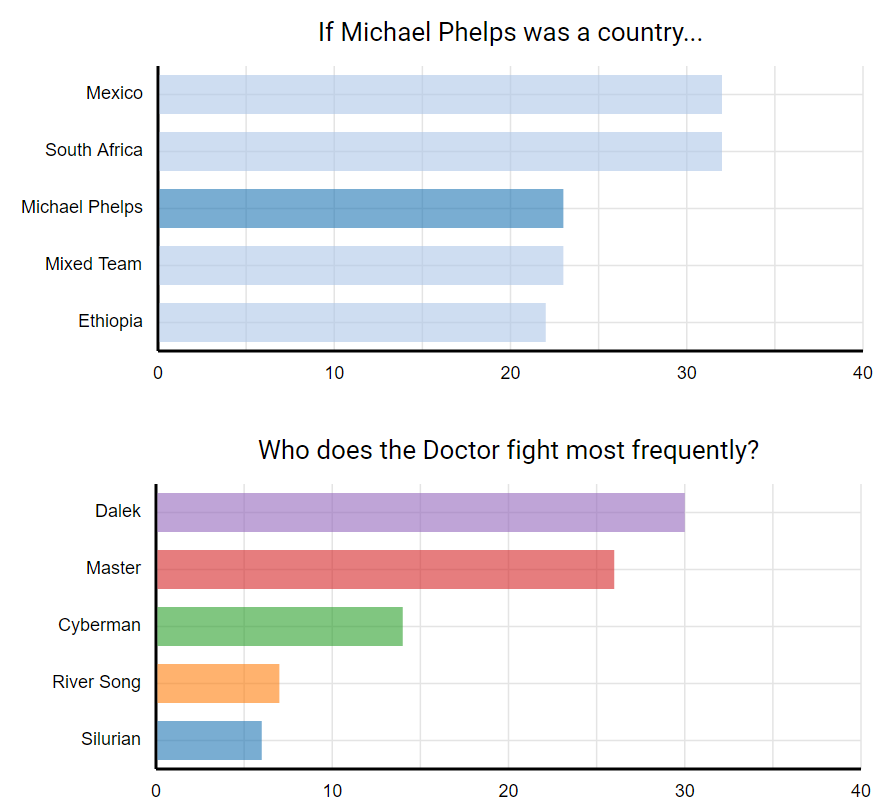
\includegraphics[width=1\columnwidth]{figures/cases}
\caption{Charts produced by two The Gamma case studies.}
\label{fig:cases}
\end{figure}

~
\newpage

% ==================================================================================================

\section{User study}
\label{sec:study}

Our goal is to develop an easy-to-learn tool that journalists and other non-programmers can use
for producing transparent data analyses. To evaluate the extent to which The Gamma achieves this,
we conduct a user study. We recruit participants among the operations and business team of a
non-profit research organization and investigate three research questions.

\paragraph{RQ1: Can non-programmers explore data with The Gamma?}
We give participants one of four simeple data exploration tasks and see if they can complete the
task using The Gamma and, possibly, how much assistance they need.

\paragraph{RQ2: Can knowledge transfer between data sources?}
Our first hypothesis is that users familiar with the iterative prompting principle will be able to
use an unfamiliar data source. In two of the tasks, participants are shown one data source and
then asked to work with a different one.

\paragraph{RQ3: Can users learn from just code samples?}
Our second hypothesis is that users can learn through precolation, i.e.~by looking at the source
code of published analyses. In one of our tasks, participants are given a code sample, but only a
minimal explanation of The Gamma environment.

\subsection{Study design}
We perform between-subjects study to evaluate the first experience of using The Gamma.
We recruit 13 participants (5 male, 8 female) from a business team
of a research lab working in various non-technical roles (project management,
partnerships, communications) including one former journalist.

We split participants into 4 groups. We first gave a brief 5 minute demonstration of The
Gamma and then asked participants to complete a task. Finally, we conducted a short semi-structured
group interview and later sent participants a follow-up questionnaire. The four tasks were:

\begin{itemize}
\item \emph{Expenditure.} Participants were given a demo using \emph{worldbank}.
  They were asked to use the \emph{expenditure} data source to compare the UK government spending
  on ``Public order and safety'' and ``Defence'' in terms of GDP.
\item \emph{Lodrs.} Participants were given a demo using \emph{worldbank}.
  They were asked to use the \emph{lords} data source (a table with House of Lords
  members expenses) to find a members representing London with the highest travel costs.
\item \emph{Worldbank.} Participants were given a minimal explanation of The Gamma environment and
  a code sample using \emph{worldbank}. They were asked to solve a different task using
  the \emph{worldbank} data source.
\item \emph{Olympics.} Participnts were given a demo using \emph{olympics}.
  They were asked to solve a more complex problem using the same data source.
\end{itemize}

We let participants work independently, but offered guidance if they got stuck for longer period of
time. Tasks \emph{expenditure} and \emph{lords} aim to answer the questions RQ1 and RQ2; the task
\emph{worldbank} aims to answer RQ1 and RQ3. In \emph{olympics}, we test RQ1 using a more complex
data source and we ask further questions to explore their understanding of the data source.

\begin{table}
  \centering
  \begin{tabular}{l l l c l}
    \toprule
      & {\small \textit{Task}}
      & {\small \textit{Kind}} & {\small \textit{Done}}
      & {\small \textit{Notes}} \\
    \midrule
    \small \#1 & \small expenditure & \small cube & \priority{50} & {\small Obtained one of two data series}\\
    \small \#2 & \small expenditure & \small cube & \priority{100} & {\small Explored furhter data series }\\
    \small \#3 & \small expenditure & \small cube & \priority{100}& {\small Explored further data series }\\
    \small \#4 & \small expenditure & \small cube & \priority{75}& {\small With hint to use another member }\\
    \small \#5 & \small expenditure & \small cube & \priority{100}& {\small Explored further data series }\\
    \small \#6 & \small worldbank & \small cube & \priority{75} & {\small With general syntax hint }\\
    \small \#7 & \small worldbank & \small cube & \priority{100} & {\small Completed very quickly }\\
    \small \#8 & \small worldbank & \small cube & \priority{100} & {\small Extra time to find data }\\
    \small \#9 & \small lords & \small table & \priority{75} & {\small  Struggled with composition}\\
    \small \#10 & \small lords & \small table & \priority{100} & {\small Completed very quickly }\\
    \small \#11 & \small lords & \small table & \priority{75} & {\small With a hint to avoid operations}\\
    \small \#12 & \small olympics & \small table & \priority{75}  & {\small With a hint to avoid operations}\\
    \small \#13 & \small olympics & \small table & \priority{75}  & {\small Hints about `then' and operations}\\
    \bottomrule
  \end{tabular}
  \caption{Overview of the work completed by individual participants. The marks denote:
    \priorityc{75} = required some guidance, \priorityc{50} = partially completed.}
  \label{tab:tasks}
  \vspace{-1em}
\end{table}

\subsection{Results}
Table~\ref{tab:tasks} summarizes the work done by the study participants.
For each participant, we record the task, the kind of data source used in the task and the
level of completion. For participants who needed assistance, the notes section details the help
given. We analyse the hints in the next section. Table~\ref{tab:quest} shows the results of the
follow-up questionnaire.

\paragraph{RQ1: Can non-programmers explore data with The Gamma?}
Three results allow us to answer RQ1 in the affirmative. First, 7 out of 9
participants agree or strongly agree that they ``found the system easy to use''. Second,
participants spent between 10 and 25 minutes (average 17 minutes) working with The Gamma and
all 12 out of 13 participants completed the task; 6 participants required some assistance,
but 3 of those faced one issue (discussed later) that could be covered in the introductory
presentation. Third, a number of participants shared positive comments in the semi-structured
interview.

Participant \#3 found the system simple, but also points out an issue about data provenance,
which we discuss later:

\begin{quote}
\emph{``This is actually pretty simple to use. You think about the logic of what you're actually
  asking and then you try to get it into the format you can. But knowing where it comes from
  would tell you how to trust it.''}
\end{quote}

Similarly, participant \#2, notes that The Gamma alleviated their unease about code:

\begin{quote}
\emph{``For somebody who does not do coding or programming, this does not feel that daunting.
  It's not like you're giving me large screen full of code, which is reassurring.''}
\end{quote}

Finally, participant \#5 suggested the system could be used as an educational tool for teaching
critical thinking with data. They answer a follow-up question about what training materials would
the students need as follows:

\begin{quote}
\emph{``I don't think they'd need more than 5 minute video (..) this is the data
  source, this is what's in there.''}
\end{quote}

\paragraph{RQ2: Can knowledge transfer between data sources?}
Our study does not conclusively answer RQ2. There is some evidence in favor of a positive answer.
In the practical part, two of the tasks (\emph{expenditure} and \emph{lords}) used a different data
source in the introductory presentation than the one that the participants were asked to use.
Participants were able to complete those tasks, although \emph{lords} has been more challenging
as it involves a more complex data source. In the interview, participant \#2 also gives a positive
answer:

\begin{quote}
\emph{``I found it quite easy to translate what you showed us in the demo to the new dataset.
   I though it was quite easy to just get how that works.''}
\end{quote}

Negative evidence is offered by the follow-up questionnaire. When asked
whether they would know how to approach a task using a new data source, 5 out of 9 participants
diagree or strongly disagree that they would know how to approach it without any further guidance.
Participants did not believe that knowledge can easily transfer to another
data source.

\paragraph{RQ3: Can users learn from just code samples?}
A positive answer to RQ3 is supported by the \emph{worldbank} task results, the follow-up questionnaire
and interview comments. In the task, participants were given only a
minimal demo of the iterative prompting principle together with print-out of 2 code samples.
All three were able to complete a related task using the same data source. In the follow-up
questionnaire, only 2 out of 9 participants disagree or strongly disagree that
they would know how to approach a task using an unfamiliar data source when given ``a number
of code samples''.

In the semi-structured interview, participants were asked what would be the most useful format
of educational material about The Gamma (code samples, video tutorials, etc.).
Participant \#7 noted that \emph{``a video would just be this [i.e.~a code sample] anyway''}, while
participant \#13 (former journalist) answered:

\begin{quote}
  \emph{``I think providing one video of one example is good and maybe a couple of little examples
  of code wher people can see the kind of things you can do.''}
\end{quote}

This is aligned with our design goal. Once the user understands the iterative prompting principle
(which can be done through a video tutorial), they can learn how to use any specific data source
just from code samples.

\subsection{Further observations}
In this section, we briefly discuss a number of observations about The Gamma design that
emerged from the study, some of which suggest ways of improving the system.

\paragraph{Making complex things possible may hurt}
As discussed earlier, The Gamma language supports operations such as \ikvd{take(5)}. Most type
providers never generate those, but the provider for working with tabular data is an exception.
When filtering data, the provider allows specifying a condition on numerical attributes such as
\ikvd{olympics.\textquotesingle filter data\textquotesingle.\textquotesingle Year is greater than\textquotesingle(2004)}.

Three participants (\#11, \#12, \#13) struggled to complete a task, because they
initially attempted to use those operations. However, those violate the iterative prompting
principle as one cannot type `.' after \ikvd{\textquotesingle Year is greater than\textquotesingle}.
This suggests that we should avoid operations in type providers for data access, even if it
limits the expressive power of the type provider.

\paragraph{Benefits and drawbacks of text}
The Gamma is based on text to aid transparency. Text hints that there is no hidden state and
the reader sees the full code. The study suggests that using a text editor has both
benefits and drawbacks compared to alternatives such as structured editors~\cite{structure-based,livenut,lamdu}.
Most participants had no difficulty navigating around source code, making edits or deleting code
fragments, which is arguably harder in an unfamiliar structured editor.

We observed two issues in the study. Participant \#2 struggled with correct indentation, starting a second command
with more indentation than needed and participant \#6 had a syntax error in an unrelated command,
which prevents charts from rendering. Some participants used the text editor effectively,
e.g.~participant \#5, who used copy-and-paste to fetch the same data series for multiple countries.

\begin{table}
  \centering
  \begin{tabular}{p{19em} c c}
    \toprule
      {\small \textit{Questionnaire item}} & {\small \textit{Avg}} & {\small \textit{Sdv}} \\
    \midrule
    \small Considering your experience \& possible use of The Gamma:\\
    \small \quad I found the system easy to use. & \small 2.11 & \small 0.87\\
    \small \quad Journalists will be able to use it to analyse data. & \small 2.67 & \small 1.05\\
    \small \quad Readers will be able to critically examine the analyses. & \small 2.44 & \small 0.68\\
    \small Thinking about the usability of the system:\\
    \small \quad The resulting programs are easy to understand. & \small 2.33 & \small 0.82\\
    \small \quad The text editor for creating them was easy to use. & \small 2.33 & \small 0.94\\
    \small \quad Finding the right item in the auto-complete was easy. & \small 2.56 & \small 1.42\\
    \small I would know how to approach a task using a new data source\\
    \small \quad If given a comprehensive video tutorial. & \small 2.00 & \small 1.24\\
    \small \quad If given a number of code samples. & \small 2.78 & \small 1.13\\
    \small \quad Without any further guidance. & \small 3.56 & \small 1.17\\
    \bottomrule
  \end{tabular}
  \caption{Summary of follow-up questionnaire responses using
    a 5-point Likert scale (1 = strongly agree, 5 = strongly disagree) over 9 subjects.}
  \label{tab:quest}
\end{table}

\paragraph{How users understand the `then' member}
When interviewing participants who worked with a tabular data source, we
asked about their understanding of the \ikvd{then} member. This is a regular member generated by the
type provider (i.e.~not a keyword), but it has a special meaning. Consider
the following example which calculates the average travel expenses and total number of
representatives per county using the UK House of Lords expenses data:

\begin{thegamma}
expneses.'group data'.'by County'
  .'average Travel Costs'.'count distinct Name'.then
\end{thegamma}

The \ikvd{then} member is used to complete a part of a query where the user can continue
adding items to build a list. Here, we select two aggregations to be calculated for each
county before choosing \ikvd{then} and applying other operations such as sorting.

Two participants (\#12 and \#13) initially thought that \ikvd{then} is used to split a command
over multiple lines, but rejected the idea after experimenting and noting that they can insert
line breaks elsewhere. One correctly concluded that it ``allows us to chain together the
operations'' of the query. Participant \#13 needed a hint about using the
\ikvd{then} member and later reflected:

\begin{quote}
  \emph{``When you explained about the `dot then' that was a really useful thing to know.
  When I found that, I was like this is fine, this is doable. If I knew this from the start,
  it would [have been easier].''}
\end{quote}

This comment summarizes an important fact. Although iterative prompting allows the users to start
exploring new data sources, the domain specific languages used by more complex data sources have
their own design principles that users need to understand to use the data source effectively.

\subsection{Conclusions}
The motivation behind The Gamma is to make simple programmatic data exploration accessible to
journalists and other non-experts. Main-stream programming languages have the benefit of
reproducibility and transparency, but are difficult to use. Our study shows that non-experts
are able to solve basic data exploration tasks using The Gamma. When asked whether The Gamma
is something that journalists could learn how to use, participant \#13 (a former journalist) answered:

\begin{quote}
\emph{``Yeah, I think so. There's a lot of effort going into data journalism that
  programming could make much quicker, but I was always nervous about code. (...)
  Something like this would really simplify things.''}
\end{quote}

The Gamma is based on the iterative prompting principle which lowers the barrier to entry, but
it is worth noting that it does not fully eliminate complexity involved in data querying.
Instead, it provides a way of structuring the complexity. Iterative prompting makes it easy to
get started, but complex data sources will inevitably require additional learning. The Gamma
makes this easier by allowing users to learn from published code samples.
\newpage
~
\newpage

% ==================================================================================================

\section{Discussion}

Data provenance (where data comes from)
What are the data sources availbale (how to start)?

\subsection{Study limitations}
exploratory in nature so we do not make any quantitative claims about effects

not comparing against other systems

\subsection{Design principles}
How well did we do wrt design principles?

\subsection{Design issues}
future challenges and limitations of the model - such as issues when modifying code
in the middle of the call chain

\section{Conclusions}

\newpage
~
\newpage

\section{Acknowledgments}
Yo

% BALANCE COLUMNS
\balance{}

% REFERENCES FORMAT
% References must be the same font size as other body text.
\bibliographystyle{SIGCHI-Reference-Format}
\bibliography{paper}


\end{document}

%%% Local Variables:
%%% mode: latex
%%% TeX-master: t
%%% End:
